% Preámbulo
\documentclass[stu, 12pt, letterpaper, donotrepeattitle, floatsintext, natbib]{apa7}
\usepackage[utf8]{inputenc}
\usepackage{comment}
\usepackage{marvosym}
\usepackage{graphicx}
\usepackage{float}
\usepackage[normalem]{ulem}
\usepackage[spanish]{babel} 
\usepackage{lastpage} %para le formato que quiere la profe QUITAR SI QUIERES OG APA7
\usepackage{ragged2e} %para le formato que quiere la profe QUITAR SI QUIERES OG APA7
\usepackage{indentfirst} %para le formato que quiere la profe QUITAR SI QUIERES OG APA7
\usepackage{multirow,booktabs,setspace,caption} %formato de figuras APA
\DeclareCaptionLabelSeparator*{spaced}{\\[2ex]}
\captionsetup[figure]{textfont=it,format=plain,justification=justified,
  singlelinecheck=false,labelsep=spaced,skip=0pt}

\selectlanguage{spanish}
\useunder{\uline}{\ul}{}
\newcommand{\myparagraph}[1]{\paragraph{#1}\mbox{}\\}

\rfoot{Página \thepage \hspace{1pt} de \pageref{LastPage}}%QUITAR SI QUIERES OG APA7 
\rhead{} %QUITAR SI QUIERES OG APA7
\setcounter{secnumdepth}{3} %permite enumerar las secciones QUITAR SI QUIERES OG APA7
\setlength{\parindent}{1.27cm} %sangria forzada QUITAR SI QUIERES OG APA7

% Portada
\thispagestyle{empty}
\title{\Large Principales Ciclos Biogeoquímicos}
\author{Abraham Jhared Flores Azcona} % (autores separados, consultar al docente)
% Manera oficial de colocar los autores:
%\author{Autor(a) I, Autor(a) II, Autor(a) III, Autor(a) X}
\affiliation{Instituto Tecnológico de Tijuana}
\course{ACD-0908SC5C Desarrollo Sustentable}
\professor{M.C. Trinidad Castro Villa}
\duedate{20 de septiembre de 2021}

\renewcommand\labelitemi{$\bullet$}

\begin{document}
\maketitle


% Índices
\pagenumbering{arabic}
    % Contenido
\renewcommand\contentsname{Contenido}
\tableofcontents
\renewcommand{\listfigurename}{Figuras}
\listoffigures

% Cuerpo 
    %NOTA: PARA CITAR ESTILO "Merts (2003)" usar \cite{<nombre_cita_bib>}
    %                        "(Metz, 1978)" usar \citep{<nombre_cita_bib>}
\newpage
\section*{Introducción}
\addcontentsline{toc}{section}{Introducción}
Como \begin{justifying}
    se ha estado explorando en la materia, uno de los aspectos de estudio priomrdiales es del Ecosistema y sus mecanismos. Como este es un sistema dinámico
    tan complejo, los avances académico/científicos han podido generalizar ciertos procesos vitales para el buen funcionamiento del Ecosistema, que son los ciclos biogeoquímicos de los cuales
    se explican en la redacción; esto incluye su definición, características y los ciclos principales con la finalidad de aumentar nuestro panorama de conocimiento para poder
    comprender de mejor manera el sistema en el cual habitamos.\par
\end{justifying}
\vspace{\baselineskip}
\section{Principales Ciclos Biogeoquímicos}
\subsection{Definición de un Cíclo Biogeoquímico}
De \begin{justifying}
    manera simple, un cíclo biogeoquímico es el reciclaje de materia inorgánica entre los organismos vivos y su entorno no-vivo \citep{openstax-no-date}.  
    Estos ciclos se asocian principalmente con las moléculas organicas (formadas con Carbono, Hidrógeno, Nitrógeno, Oxígeno, Fosforo y Sulfuro) que toman formas
    químicas distintas y pueden existir por largos periodos de tiempo en la atmósfera, en la tierra, en el agua o debajo de la superficie del planeta Tierra.
Aunado a esto, los procesos geológicos como la erosión, drenado de agua, el movimiento de las placas tectónicas, y el clima, estan involucrados en el ciclado de los
    elementos terrestres. Es por ello que los ciclos biogeoquímicos se apoyan de los campos de la Geología y la Química.\par
\end{justifying}
\vspace{\baselineskip}
\subsection{Cíclo del Carbono}
Este \begin{justifying}
    cíclo mueve el Carbono de la atmósfera hacia las plantas. Dentro de la atmósfera, el Carbono se acopla al Oxígeno para formar Dióxido de Carbono. Con el proceso de la
    fotosíntesis, el Dioxido de Carbono es tomado del aire para producir comida hecha de Carbono para el crecimiento de la planta. Con las cadenas alimenticias, el susodicho elemento
    se mueve a los animales que consumen las plantas y los consumidores de estos animales obtienen el Carbono de esta manera. Con la defunción de los especímenes, el Carbono regresa a
    la tierra donde se convertirán en combustibles fósiles eventualmente \citep{openstax-no-date}.\par
\end{justifying}
\vspace{\baselineskip}
\begin{figure}[H]
    \caption{\emph{Ciclo del Carbono}}
    \centering
    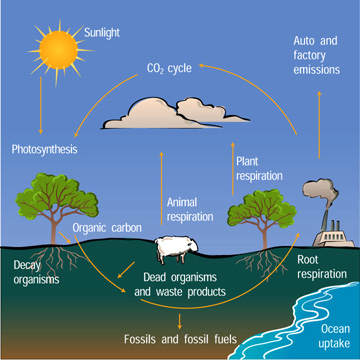
\includegraphics[width=14cm,height=10cm]{carbon.jpg}
    \bigskip
    \\\small\textit{Nota}. Tomado de \cite{openstax-no-date}. %citar el de lumen
\end{figure}
%\vspace{\baselineskip}
Es \begin{justifying}
    importante destacar que el intercambio del Dióxido de Carbono de la atmósfera y superficie terrestres ocurre naturalmente ciertos años. Esto se copla con el ciclado lento en la vegetación terrestre,
    el terreno y el oceano alto; específicamente las tierras profundas y el mar profundo. La emisión de Carbono es lo que ha aumentado el contenido atmosférico del Dióxido de Carbono \cite{stocker-2013}. 
\end{justifying}
\vspace{\baselineskip}
\subsection{Cíclo del Nitrógeno}
A \begin{justifying}
    pesar de que este elemento se encuentra en distintas macromoléculas biológicas, el poder ingresar Nitrogeno a los organismos vivos es dificil. Las celulas procariotas son las que juegan roles esenciales en este ciclo
    al transformar Nitrogeno en varias formas para sus necesidades propias, que terminan beneficiando a otros organismos de manera indirecta; este proceso se conoce como Fixación de Nitrogeno que consiste en Cyanobacterias
    encontradas en ecosistemas acuaticos que arreglan el Nitrogeno Inorgánico en Amoniaco el cual es facilmente incorporable en macromoléculas biológicas \citep{unknown-author-no-date}.\par
\end{justifying}
Dicho \begin{justifying}
    Nitrogeno arreglado es convertido eventualmente de Nitrogeno Orgánico a Gas Nitrógeno por microbios a travéz de tres pasos: amonificación, nitrificación y desnitrificación. Con la amonificación ciertas bacterias y fungi 
    convierten el desecho nitroso en Amoniaco, eventualmente dicho compuesto es oxidado en Nitrito (nitrificación), de ahí en Nitrato (desnitrificación).\par
\end{justifying}
\vspace{\baselineskip}
\begin{figure}[H]
    \caption{\emph{Ciclo del Nitrogeno}}
    \centering
    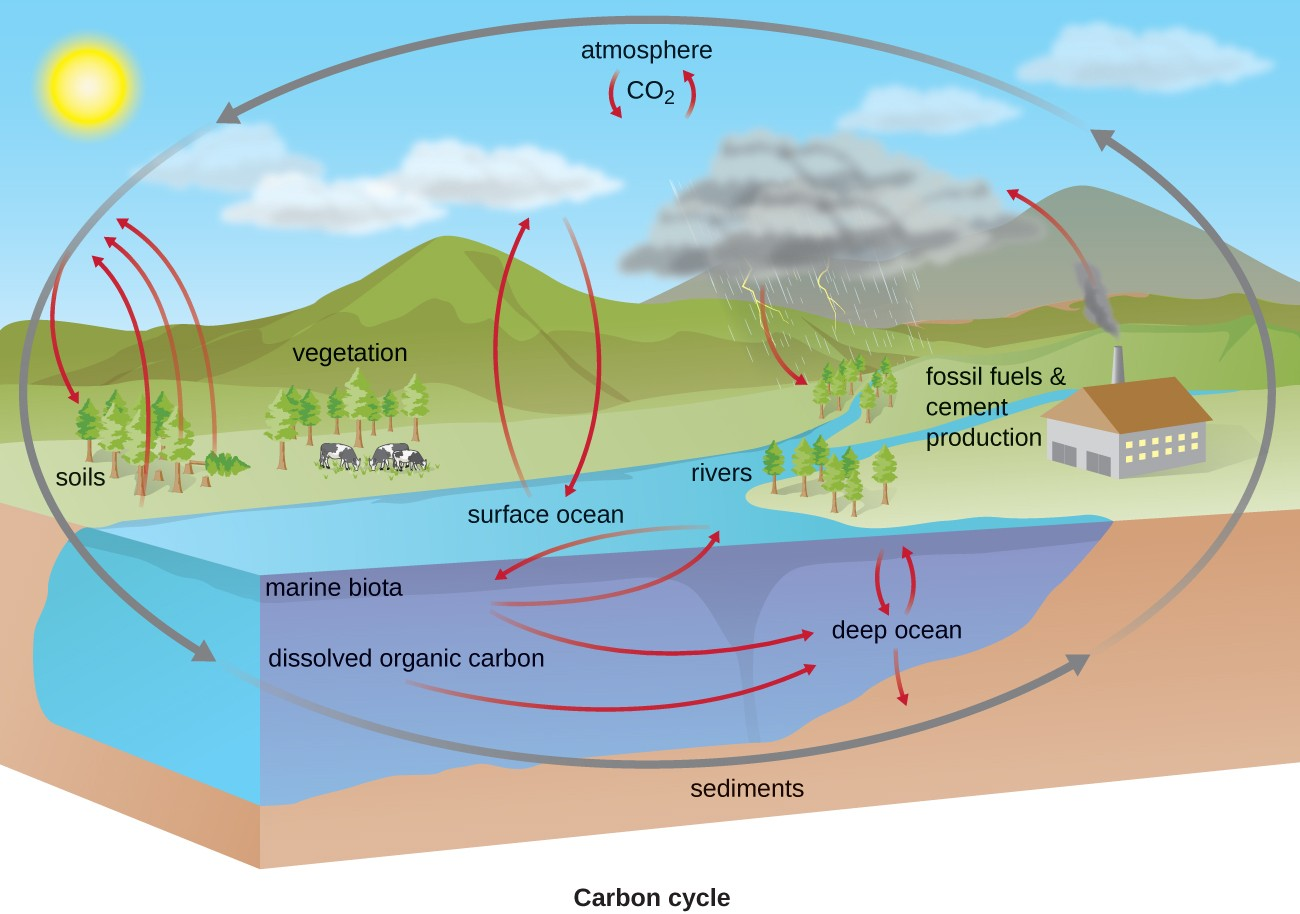
\includegraphics[width=14cm,height=7cm]{nitrogeno.jpg}
    \bigskip
    \\\small\textit{Nota}. Tomado de \cite{openstax-no-date}. %citar el de lumen
\end{figure}
La \begin{justifying}
    creación del Nitrogeno reactivo por el proceso Haber-Bosch sumado a la combustión de combustibles fósiles y la Fixación Agricutural Biológica de Nitrogeno han impactando los balances de radiación de la Tierra; dicho equilibrio
    se ha roto con la Revolución Industrial \citep{stocker-2013}. %citar al articulon
    La contaminación de estos compuestos de nitrogeno como el Oxido Nitroso se puede apreciar al mirar al cielo y notar el color rojizo-cafe que llamamos smog \cite{unknown-author-no-date}.\par %citar al de scied
\end{justifying}
\vspace{\baselineskip}
\subsection{Cíclo del Sulfuro}
Relacionado \begin{justifying}
    con otro elemento esencial para las macromoléculas de los organismos vivos tales como la formación de proteinas.
    Las bacterios fotosintéticas anoxigénicas así como otras usan el Sulfito de Hidrógeno como un donado de electrones, oxidando al Sulfito en Sulfuro elemental, y de ahí en Suldato. La decomposición de los organismos difuntos dada por fungi y bacterias remueven los grupos de Sulfuro
    de los aminoacidos, produciendo Sulfito de Hidrógeno, el cual retorna el Sulfuro inorganico al entorno \citep{openstax-no-date}.\par
\end{justifying}
\vspace{\baselineskip}
\begin{figure}[H]
    \caption{\emph{Ciclo del Sulfuro}}
    \centering
    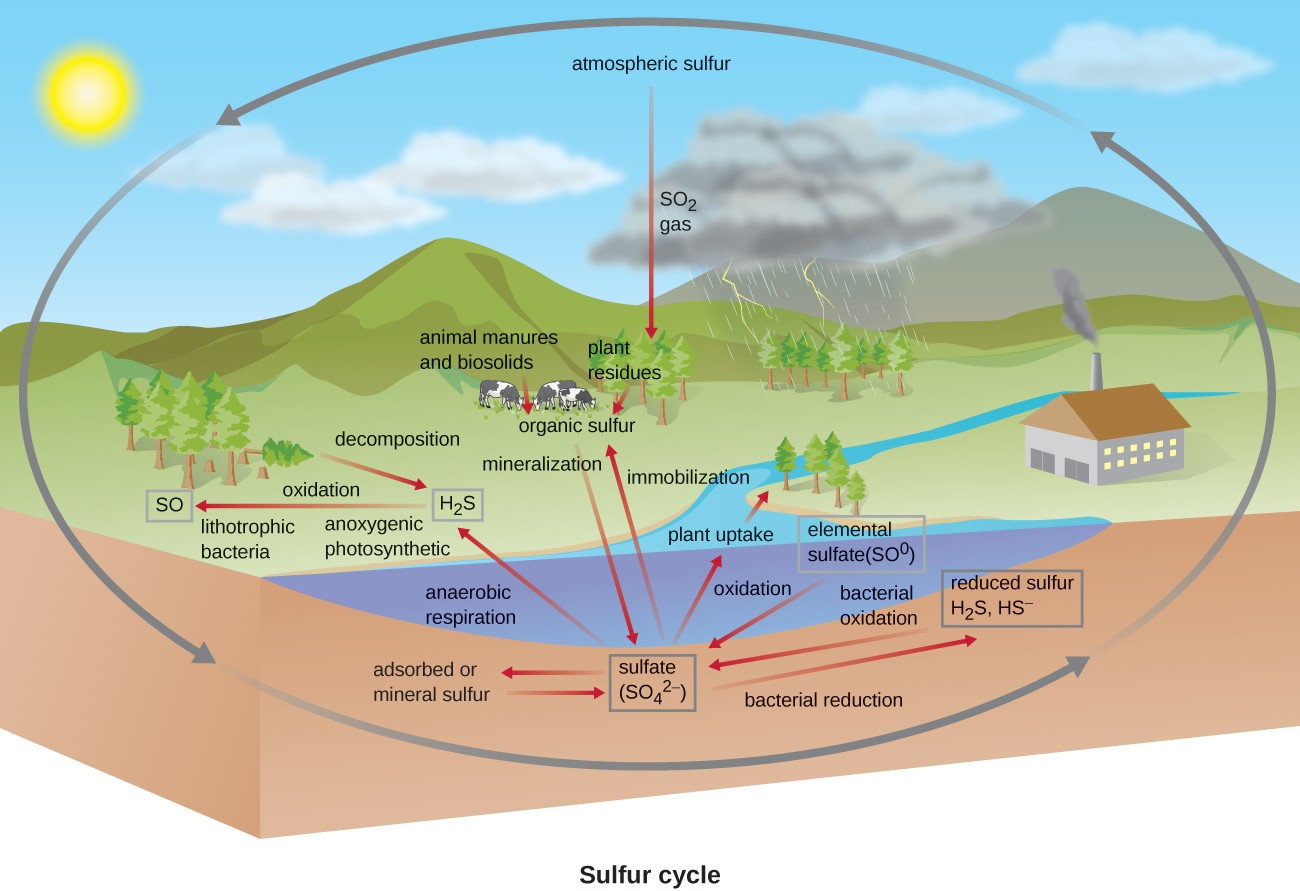
\includegraphics[width=14cm,height=7cm]{sulfato.jpg}
    \bigskip
    \\\small\textit{Nota}. Tomado de \cite{openstax-no-date}. %citar el de lumen
\end{figure}
\section{Concatenación de las Entradas y Salidas de Energía en el Ecosistema}
La \begin{justifying}
    energía, al contrario de la materia, no puede ser reciclado en los ecosistemas. En vez de, el flujo de energía dentro del ecosistema es de una sola dirección la cual generalmente sucede de la luz a calor.
    Dicha energía usualmente entra como luz solar y es capturada en forma química por los organismos capaces de la fotosíntesis. De ahí, la energía es pasada entre el ecosistema, cambiando de forma ya que los organismos
    metabolzan, producen desecho, se comen unos a otros, y eventualmente, mueren y se descomponen.
    Cada vez que la energía cambia de forma, alguna porción de esta se convierte en calor. Este calor cuenta como energía pero de manera general los organismos vivos no pueden utilizarla como una fuente energética. Ultimadamente,
    la energía que entró al ecosistema como luz solar es disipada como calor y es irradiada hacia el espacio \citep{khan-academy-no-date}.\par
\end{justifying}
\vspace{\baselineskip}
\begin{figure}[H]
    \caption{\emph{Ejemplo de Entradas y Salidas de Energía: Cadena Alimenticia}}
    \centering
    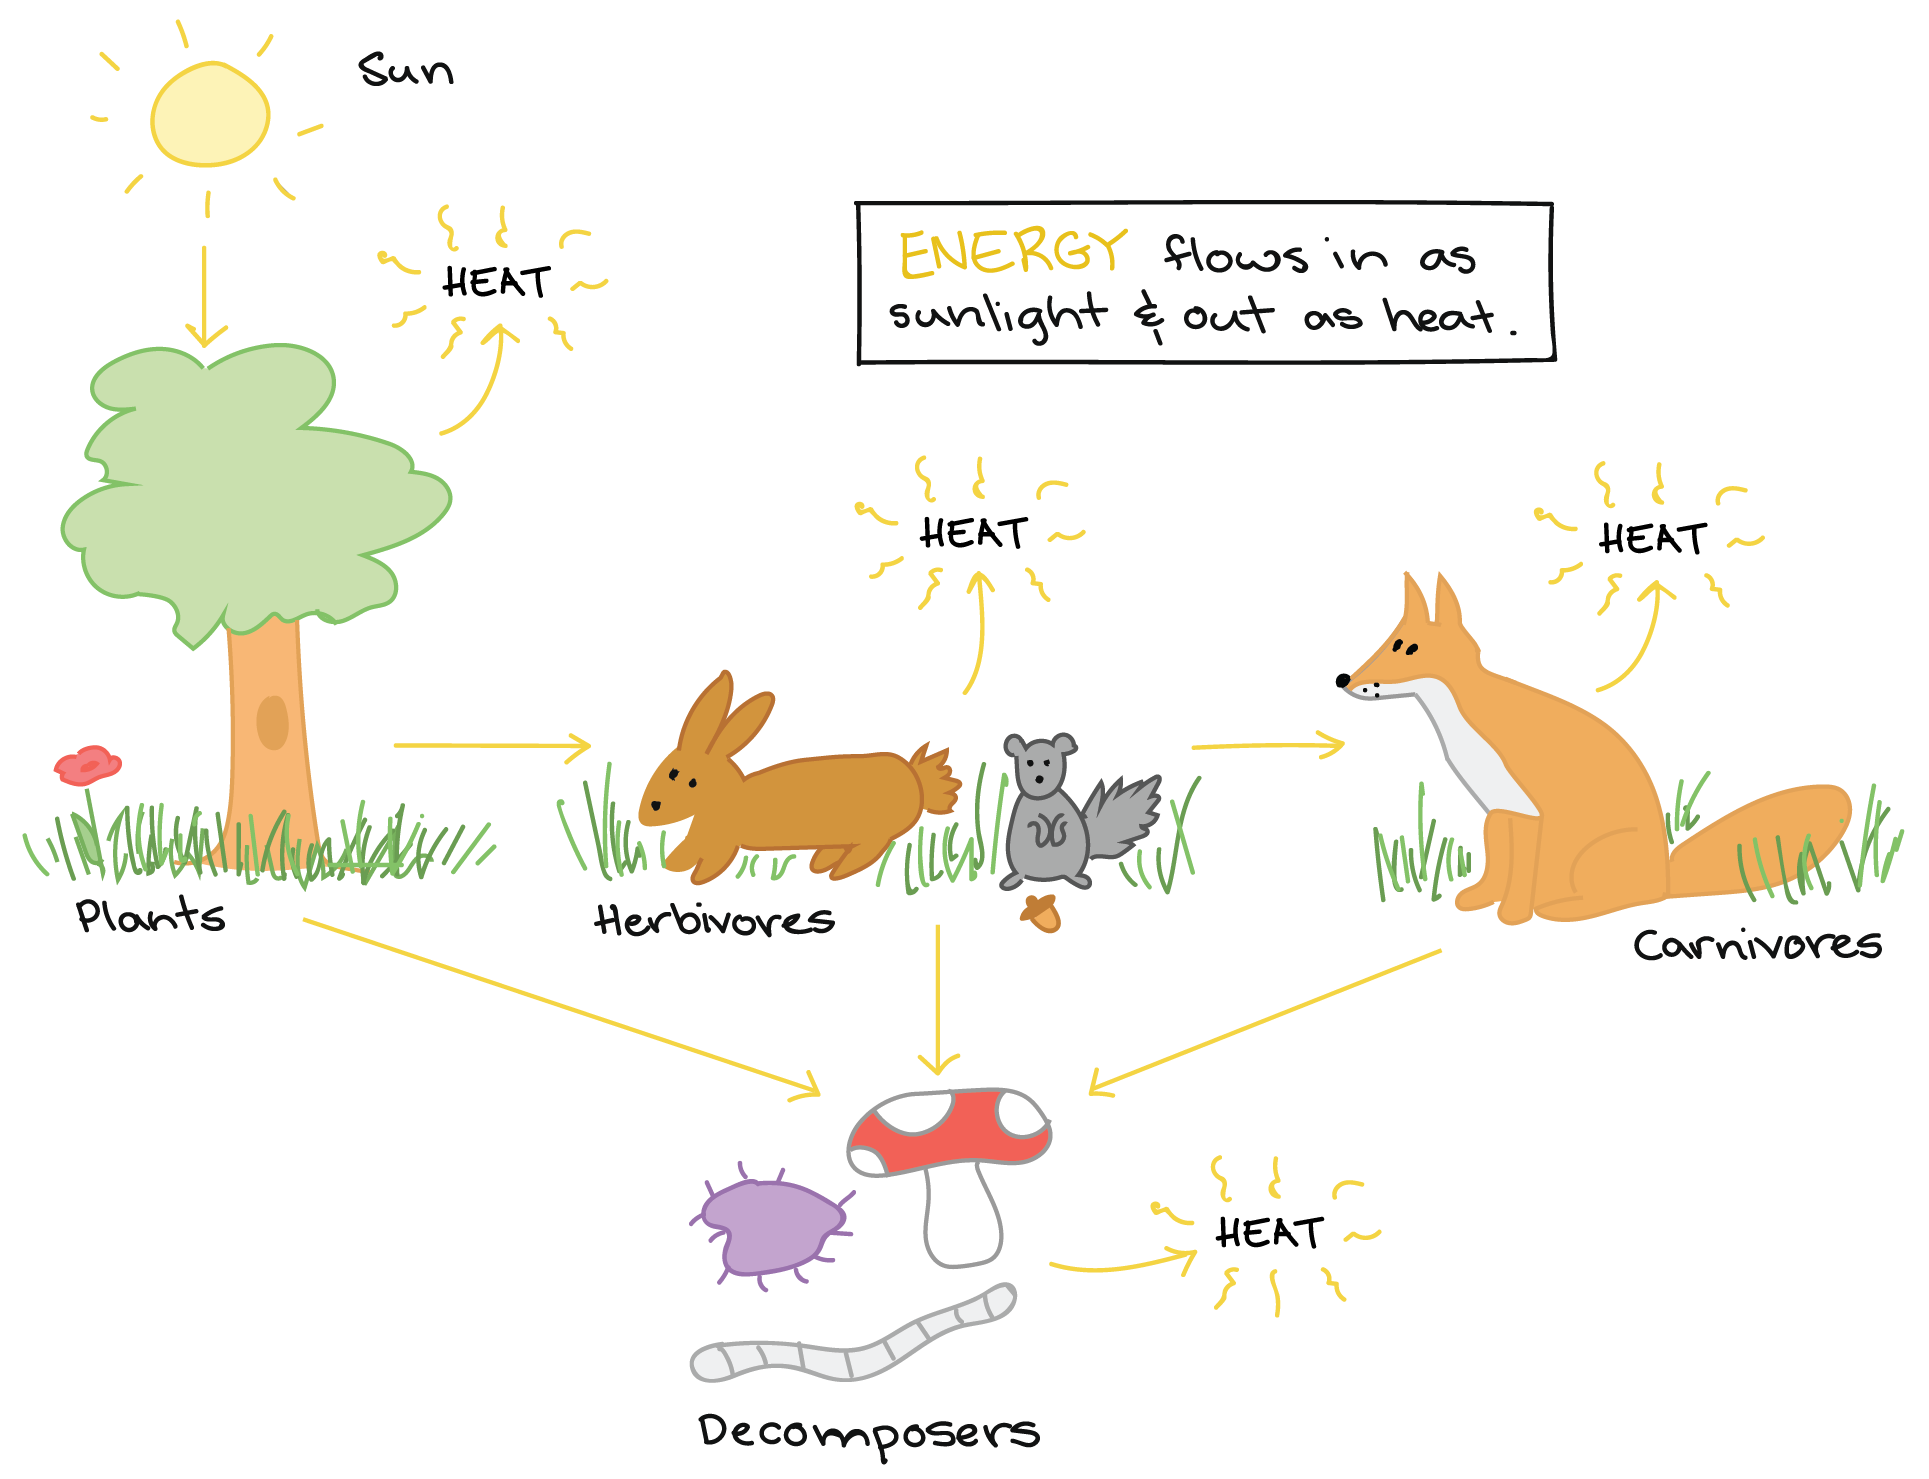
\includegraphics[width=14cm,height=10cm]{evenflow.png}
    \bigskip
        \\\small\textit{Nota}. La principal fuente de energía proviene de la luz solar. Tomado de \cite{khan-academy-no-date}. %citar el de lumen  
\end{figure}
\section*{Conclusión}
\addcontentsline{toc}{section}{Conclusión}
Como \begin{justifying}
    todo sistema complejo, los ecosistemas cuentan con distintos mecanismos los cuales permiten la subsistencia de estos, como los expuestos en la redacción, nos permiten comprender de manera generalizada
    estos engranajes que permiten a esta gran maquinaria el poder funcionar de manera plena. Por ello es relevante considerar las afectaciones humanas para investigar el mejor punto de equilibrio tanto para la raza humana, sus acciones
    y el ecosistema.\par
\end{justifying}

\newpage
% Referencias
\setcounter{secnumdepth}{0} %permite enumerar las secciones QUITAR SI QUIERES OG APA7
\renewcommand\refname{\textbf{Referencias}}
\bibliography{referencias}

\end{document}